\newgeometry{left=4.5cm, right=4.5cm,bottom=4cm, top=4cm}
\chapter{The ATLAS Detector at the LHC}\label{chap:detector}
 \vspace{0.5cm}

The Large Hadron Collider (LHC) located at the European Organization for Nuclear Research (CERN) in Geneva, Switzerland,
is  the largest particle collider facility in the world, colliding protons and heavy ions at so far largest centre-of-mass
energies. The ATLAS experiment is one of the several experiments 
at the LHC, taking data with a  general-purpose detector designed  to search for  a wide range of new 
physics phenomena and to perform  precision measurements of known Standard Model processes.
Proton-proton collision data recorded by the ATLAS detector in 2012  has been used for 
the search for the neutral MSSM Higgs bosons presented in this thesis.

This chapter is organised as follows: the design and performance of the LHC  are summarised in 
Section~\ref{sec:lhc}, based on~\cite{LHC},  while  a brief description of the 
 ATLAS detector  is given in Section~\ref{sec:atlas}, based on~\cite{ATLASDetector}.


\restoregeometry
\clearpage



\section{The Large Hadron Collider}\label{sec:lhc}
The LHC is a superconducting hadron synchrotron  collider. It is  installed in the tunnel of the former Large Electron-Positron collider (LEP)
with a circumference of about $27$~km.
LHC is designed to collide proton beams at a nominal centre-of-mass energy of 14 TeV and an unprecedented peak luminosity of 
$10^{34} ~ \text{cm}^{-2} \text{s}^{-1}$. It can also collide heavy ion (lead) beams carrying  an energy of 2.8 TeV per nucleon and 
a peak luminosity of $10^{27} ~ \text{cm}^{-2} \text{s}^{-1}$. 

Figure~\ref{fig:LHC} shows the layout of the CERN accelerator complex. The  protons undergo several acceleration steps before 
their injection into the LHC machine.
The a linac accelerator ($Linac\,2$) accelerates the protons to an energy of 50~MeV, after which
they are injected into the \emph{booster} and further  accelerated
to 1.4~GeV. The proton energy is increased to 25~GeV and successively to 450~GeV by means of two synchrotron accelerators, the \emph{Proton Synchrotron} (PS)
and the \emph{Super Proton Synchrotron} (SPS). Finally, two proton beams are  injected in opposite directions into the LHC ring
where they reach their final energy.

The proton beams are  housed in two separate vacuum pipes and consist of up to 2835 proton bunches, each
of them containing about $10^{11}$ protons. 
Radiofrequency cavities are employed  to accelerate the protons,
while superconducting magnets bend and focus the bunches.
The nominal bunch spacing allows for bunch crossings  every 25~ns and represents a challenge for any detector read-out electronics.

First proton-proton collisions took place at the LHC in 2010 at a centre-of-mass  energy of 7~TeV. 
The LHC was successfully delivering data during  years 2011 and 2012, increasing the  centre-of-mass  energy to 8~TeV in 2012.
Peak luminosities of about $4\times10^{33} ~ \text{cm}^{-2}\text{s}^{-2}$ and $8\times10^{33} ~ \text{cm}^{-2}\text{s}^{-2}$  have been reached 
during years 2011 and 2012 respectively.
The physics program of the LHC is driven by four major experiments which are ATLAS~\cite{ATLASDetector}, CMS~\cite{cms},
LHCb~\cite{lhcb} and ALICE~\cite{alice}. 
The ATLAS experiment recorded proton-proton collision data corresponding to an integrated luminosity of 4.57~$\text{fb}^{-1}$ 
during year 2011 and additional  20.3~$\text{fb}^{-1}$ during 2012.
Data recordered during  these two years  led among others to one of the major milestones
 in particle physics, the discovery of  a Higgs boson with a mass of about $\sim 126$~GeV.





\begin{figure}[tp]
     \begin{center}

            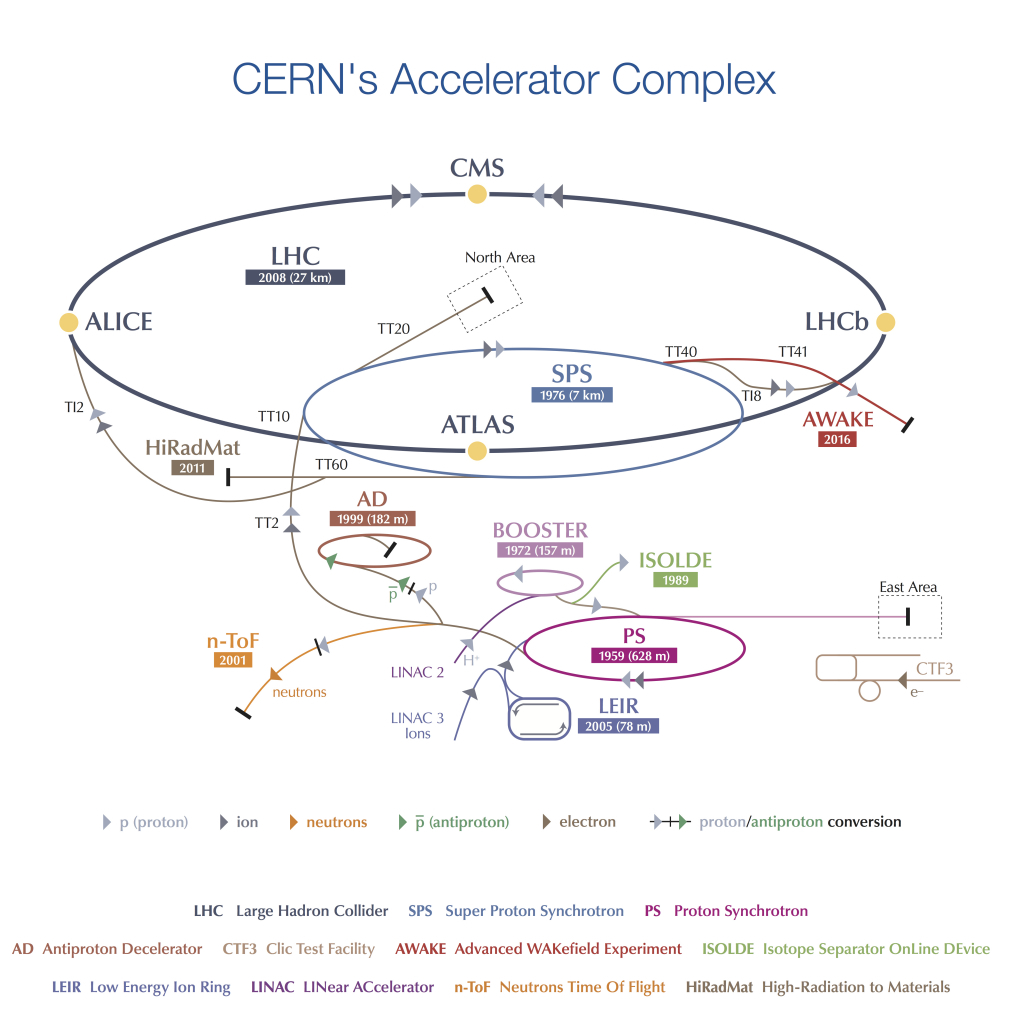
\includegraphics[width=\textwidth]{figure/LHC2.jpg}

    \end{center}
    \caption{Illustration of the CERN accelerator complex~\cite{lhcImage}. The acceleration of protons starts with Linac2 followed by the
	acceleration in the Booster. The Proton Synchrotron (PS) and the Super Proton Synchrotron (SPS) accelerate the protons further  before
	their final injection into the LHC  machine, where they acquire their final energy.}


   \label{fig:LHC}
\end{figure}


\section{The ATLAS Detector}\label{sec:atlas}
The ATLAS detector is a multi-purpose detector aiming to explore a wide range of physics 
phenomena at the Teraelectronvolt energy scales.
The physics goals drive the detector design, imposing strong requirements on particle reconstruction and 
 identification accuracy.
A schematic view of the ATLAS detector is shown in Figure~\ref{fig:atlas}, 
with its length of $44\,$m and its height of $25\,$m  is the largest detector at the LHC, it is centred around one of the LHC interaction points about
100 under ground. ATLAS consist of four sub-detectors which are installed  cylindrically around the
beam pipe, symmetrically in the forward and backward direction with respect to the proton beams.
The innermost sub-detector is the inner detector (ID), followed by the electromagnetic calorimeter, the hadronic calorimeter and finally
a muon spectrometer (MS) in the outermost layer. Each of these sub-detector is briefly described in what follows based on  Reference~\cite{ATLASDetector}.


\begin{figure}[tp]
     \begin{center}

            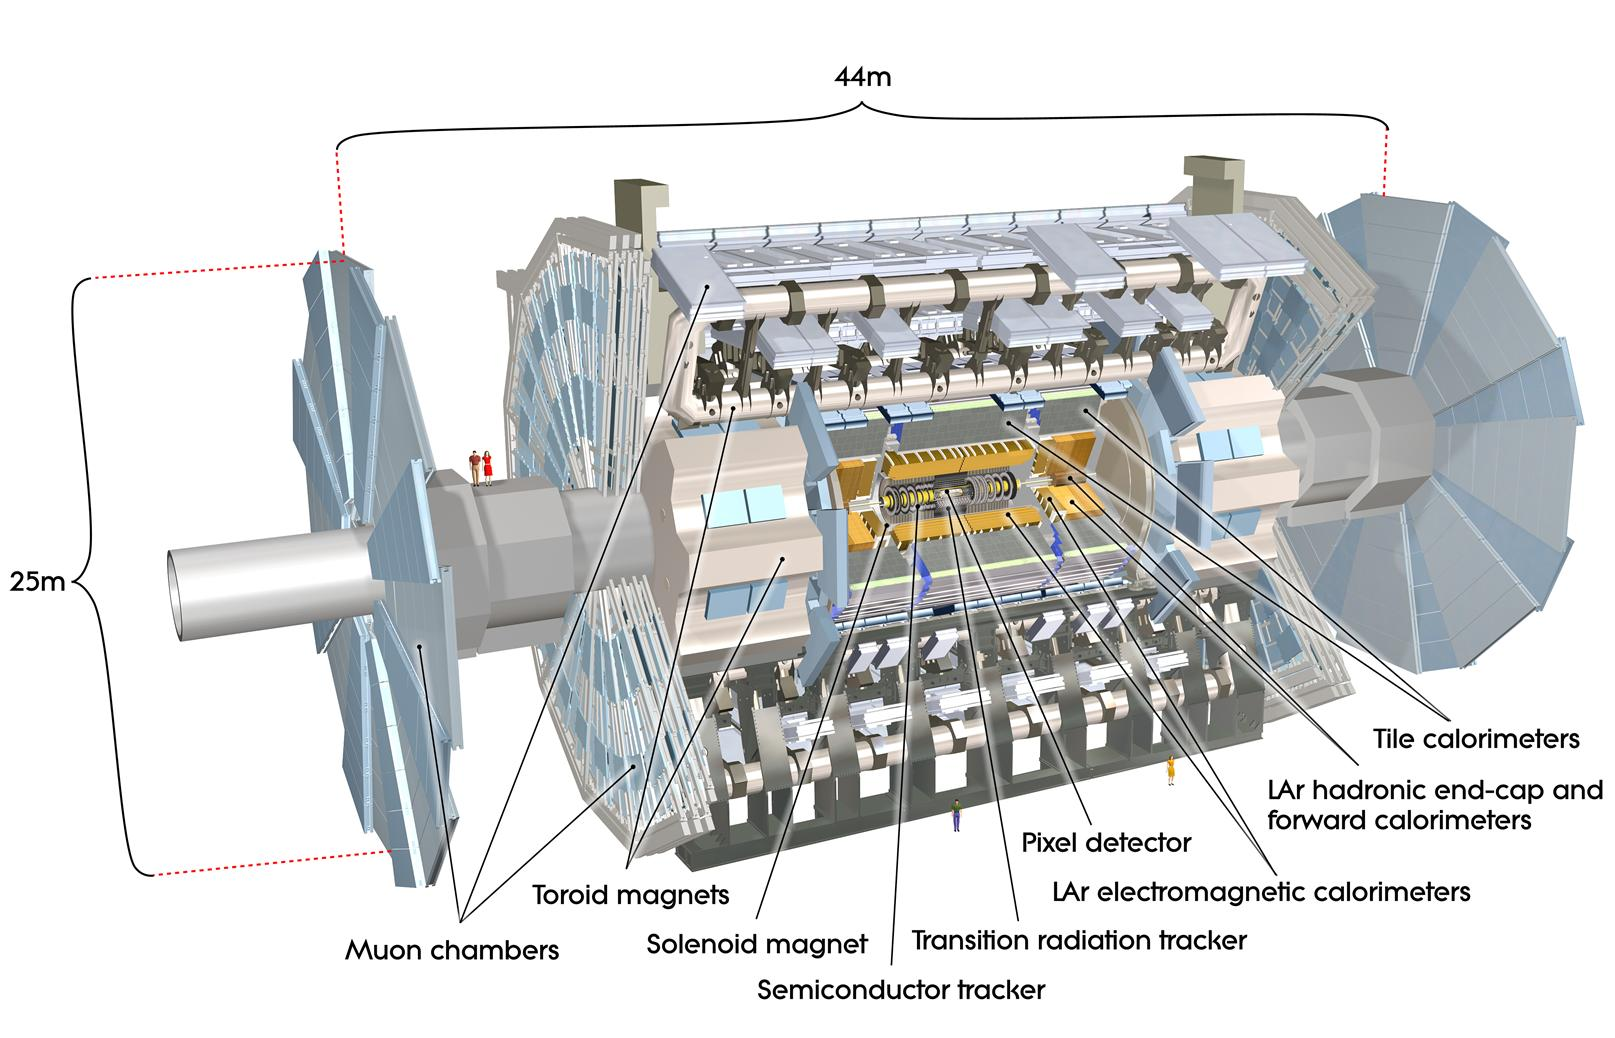
\includegraphics[width=\textwidth]{figure/ATLAS.jpeg}

    \end{center}
    \caption{Cut-away view of the ATLAS detector with its sub-detectors~\cite{ATLASDetector}.}



   \label{fig:atlas}
\end{figure}


\subsection{The ATLAS coordinate system}
The ATLAS coordinate system has its origin at the interaction point. The $z-$axis is pointing along the beam direction,
the $y-$axis  upwards and the $x-$axis towards the centre of the LHC ring. The azimuthal angle $\phi$ is defined in the transverse plane orthogonal
to the beam axis, starting from the positive side of the $x-$axis. The polar angle $\theta$ is  defined with respect to the $z-$axis.

A commonly used spatial coordinate in  collider experiments  is related to the rapidity $y$:
\begin{equation}
y ~ = ~ 1/2 \cdot \ln \left( \frac{E + p_{z}}{E - p_z} \right) \,, 
\end{equation}
where $E$ and $ p_z$ are the particle energy and the momentum component in the $z$-direction, respectively.
The difference in the rapidity of two particles is independent of Lorentz boosts along the beam axis. 
In the limit of the relative velocity $\beta$ approaching to 1 (i.e. the speed of light)
or for massless particles the rapidity corresponds to the pseudorapidity $\eta$,
\begin{equation}
\eta ~ = ~ 1/2 \cdot \ln \left( \frac{\theta}{2} \right)\,. 
\end{equation}
Based on the ATLAS detector layout, the detector is divided into the \emph{barrel} region, with a cylindrical structure, 
extended for $|\eta| \apprle 1.5$ (depending on the particular  sub-detector) 
and the \emph{endcap} region, with a disk structure, for larger~$\eta$ values. The angular separation between two particles is commonly 
quantified with $\Delta R ~=~\sqrt{\Delta \eta^2 + \Delta \phi^2}\,$, where $\Delta\eta$ and $\Delta\phi$ are the difference in pseudorapidity
and azimuthal angle of these particles, respectively.
%Given the symmetry 
%of the ATLAS detector, it is divided in two regions, barrel and endcap.

\subsection{The Inner Detector}

\begin{figure}[tp]
     \begin{center}

            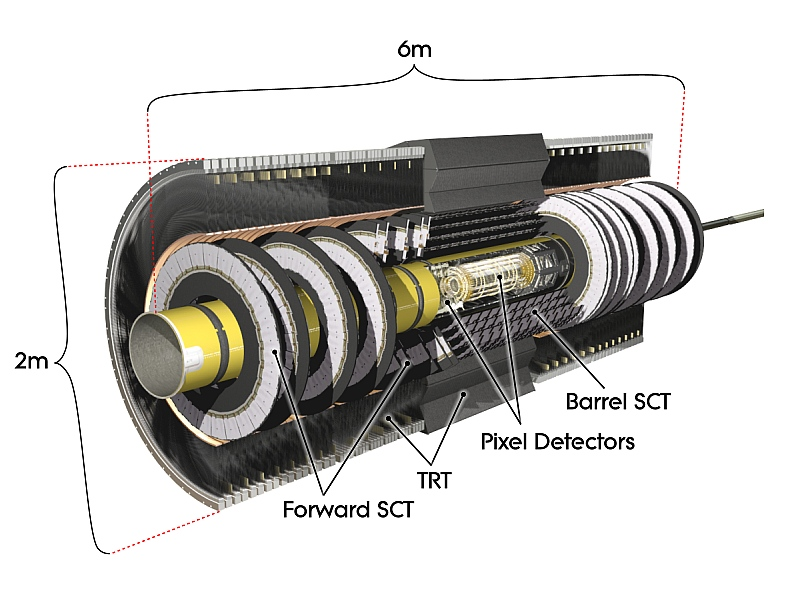
\includegraphics[width=0.7\textwidth]{figure/Inner_detector.jpg}

    \end{center}
    \caption{Cut-away view of the ATLAS inner detector~\cite{ATLASDetector}.}

   \label{fig:atlasID}
\end{figure}


The inner detector performs the reconstruction  of curved charged particles trajectories in a 2\,T solenoidal magnetic field,
providing the particles momenta as well as the position of the interaction vertices. 
The layout of the inner detector is illustrated in Figure~\ref{fig:atlasID}.
It has a total length of $5.3\,$m, a diameter of $2.5\,$m and consists
 of three independent detector modules with fine granularity
covering the pseudorapidity region $|\eta| < 2.5\,.$ The innermost inner detector module is the pixel detector
which consists of three cylindrical layers of pixel silicon sensors in the barrel and three disks in the endcap region. 
The pixel layer closest to the beam pipe is
referred to as the B-layer, since it provides crucial informations for the identification of b-quarks. 
The pixel sensors have a spatial resolution of  $10\,\mu$m in the transverse and $115\,\mu$m in the longitudinal
direction with respect to the beam pipe.

The Semi-Conductor Tracker (SCT) surrounds the pixel detector with four cylindrical layers of silicon microstrip sensors in the barrel
and nine disks in the  endcap region. The spatial resolution achieved by the SCT sensors is $17\,\mu$m in the transverse and $590\,\mu$m 
in the longitudinal direction.

The outermost inner detector module is the Transition Radiation Tracker (TRT). It is composed of $4\,$mm diameter kapton straw tubes
with a tungsten wire in their centre. The tubes are filled with a gas mixture (70\% Xe, 27\% CO$_2$
and 3\% $\text{O}_2$) which allows for the detection of transition 
radiation photons. This detector can only measure the particle position in the transverse plane.

% is t used in
%conjunction with the straw tubes of the Transition Radiation Tracker (TRT), offer these features.
%The precision tracking detectors (pixels and SCT) cover the region
%|η| < 2.5. In the barrel region, they are arranged on concentric cylinders around the beam axis
%while in the end-cap regions they are located on disks perpendicular to the beam axis. The highest
%granularity is achieved around the vertex region using silicon pixel detectors. The pixel layers are
%segmented in R − φ and z with typically three pixel layers crossed by each track. All pixel sensors
%are identical and have a minimum pixel size in R − φ × z of 50 × 400 μm2 . The intrinsic accuracies
%in the barrel are 10 μm (R − φ ) and 115 μm (z) and in the disks are 10 μm (R − φ ) and 115 μm (R).
%The pixel detector has approximately 80.4 million readout channels. For the SCT, eight strip layers
%(four space points) are crossed by each track. In the barrel region, this detector uses small-angle
%(40 mrad) stereo strips to measure both coordinates, with one set of strips in each layer parallel to
%the beam direction, measuring R − φ . They consist of two 6.4 cm long daisy-chained sensors with
%a strip pitch of 80 μm. In the end-cap region, the detectors have a set of strips running radially and
%a set of stereo strips at an angle of 40 mrad. The mean pitch of the strips is also approximately
%80 μm. The intrinsic accuracies per module in the barrel are 17 μm (R − φ ) and 580 μm (z) and in
%the disks are 17 μm (R − φ ) and 580 μm (R). The total number of readout channels in the SCT is
%approximately 6.3 million.




\subsection{The Calorimeter System}

\begin{figure}[tp]
     \begin{center}

            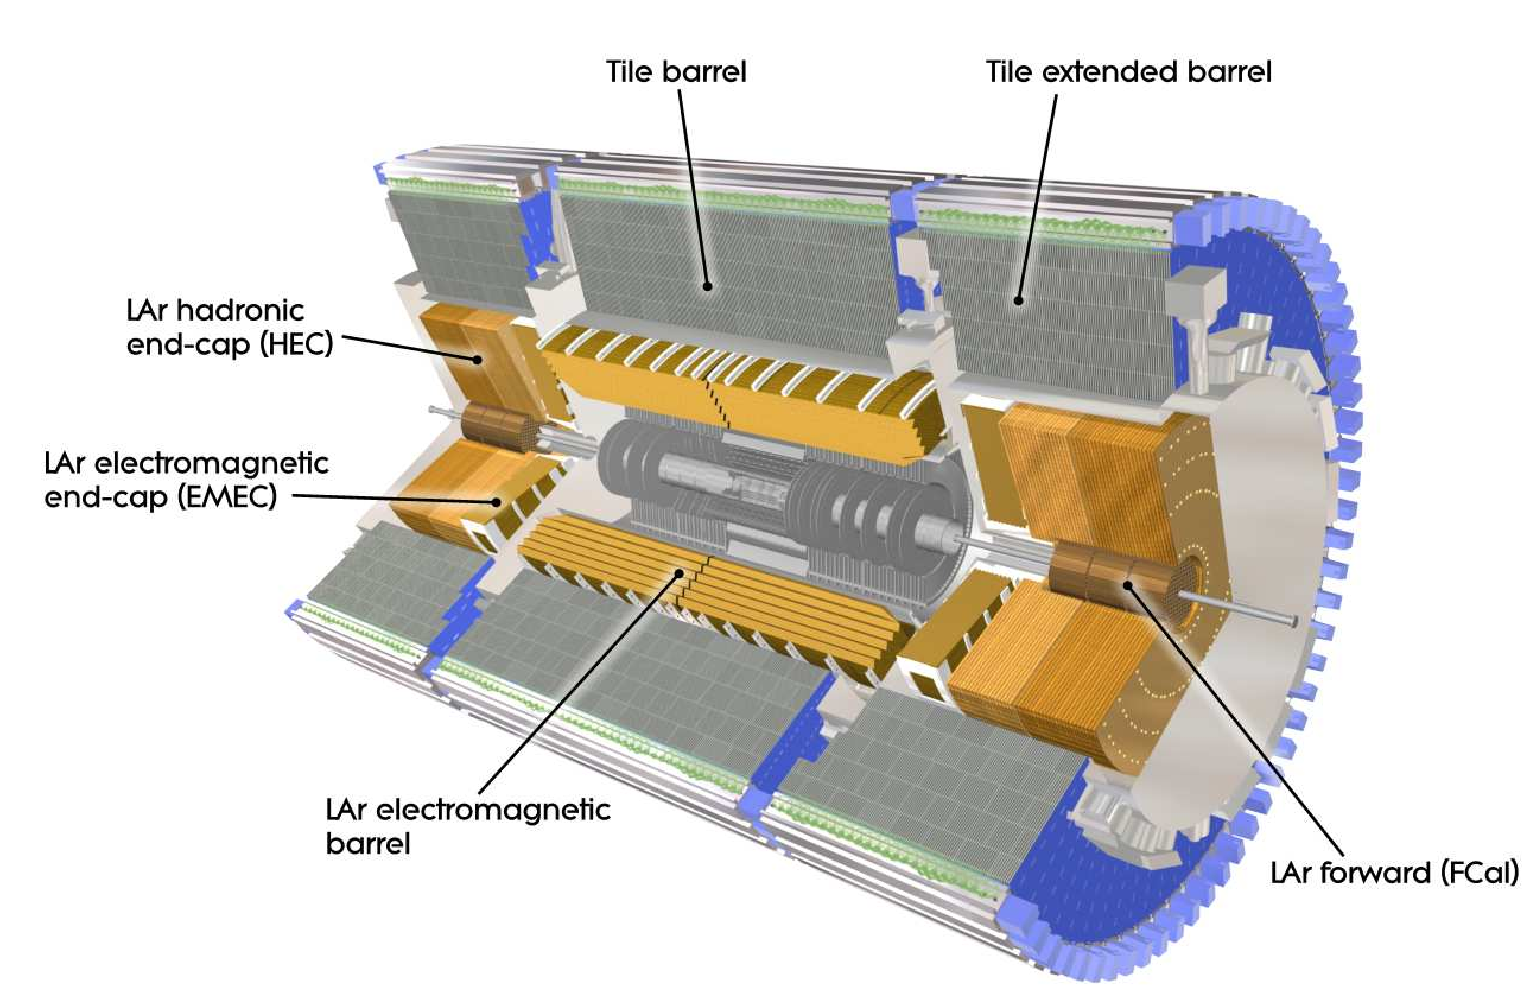
\includegraphics[width=0.7\textwidth]{figure/Calo.png}

    \end{center}
    \caption{Cut-away view of the ATLAS calorimeter system~\cite{ATLASDetector}.}



   \label{fig:atlasCal}
\end{figure}

An illustration of the ATLAS calorimeter system is shown in Figure~\ref{fig:atlasCal}. It consists of an electromagnetic calorimeter (EM) 
surrounded by a hadronic calorimeter.  These calorimeters cover the pseudorapidity 
range $|\eta| < 4.9$.
%
%using different techniques suited to the
%widely varying  radiation environment over this large $\eta-$range. 
Both  calorimeters are sampling calorimeters, built of alternating
active material which performs the detector response and a passive absorber.
The total detector material  at $\eta = 0$ corresponds to an interaction length $\lambda$ of 9.7$\,.$ 

The EM liquid-argon (LAr) calorimeter is ideally suited for the precision measurement of electron and photon
energy. Liquid argon acts as  active material while lead is used as an absorber. The EM calorimeter extends up to $|\eta| < 3.2\,.$
The total thickness of the EM calorimeter is about 22 radiation lengths in the barrel and greater than 24 in the
end-caps. It is divided in depth into three cylindrical layers each of them additionally segmented in $\eta-\phi$ cells with 
different size depending on the layer and on pseudorapidity. The $\phi$ and size of a cell rages from  0.025-0.1, while its $\eta$ size ranges 
from 0.0035-0.075\,.
The energy resolution for electrons and photons ranges from 9-22\%/$\sqrt{E}$ and from 8-14\%/$\sqrt{E}$ respectively depending on
pseudorapidity.

The hadronic calorimeter has a coarser granularity with respect the EM calorimeter and  is suited  for
reconstruction of hadronic showers (jets) and measurement of missing transverse energy. It 
is divided in three sub-detector systems which make use of several different technologies to cope 
with the $\eta$-dependent radiation environment. A tile calorimeter covers the pseudorapidity range up to $|\eta| < 1.7\,$. 
Scintillating tiles are employed as active material and steel as an absorber. 
In the forward region, the hadronic calorimeter is instrumented with a LAr hadronic endcap calorimeter (HEC)
which extends up to $|\eta| < 3.2$ and uses argon as an active material and copper as an absorber. 
The most forward region with  $3.1 <|\eta| < 4.9$ is instrumented  with a 
liquid argon Forward CALorimeter (FCAL), 
%this provides clear benefits in terms of uniformity of the calorimetric coverage as well as
%reduced radiation background levels in the muon spectrometer. 
which is divided in three modules. In the module closest to the interaction point, copper is used as absorber material, 
while the other two modules employ tungsten.
The jet energy resolution in the barrel is of about 15\% for jets of $\pt=50$~GeV and it is of about 7\% for jets of $\pt=1$~TeV~\cite{jer}.


\subsection{The Muon Spectrometer}
\begin{figure}[tp]
     \begin{center}

            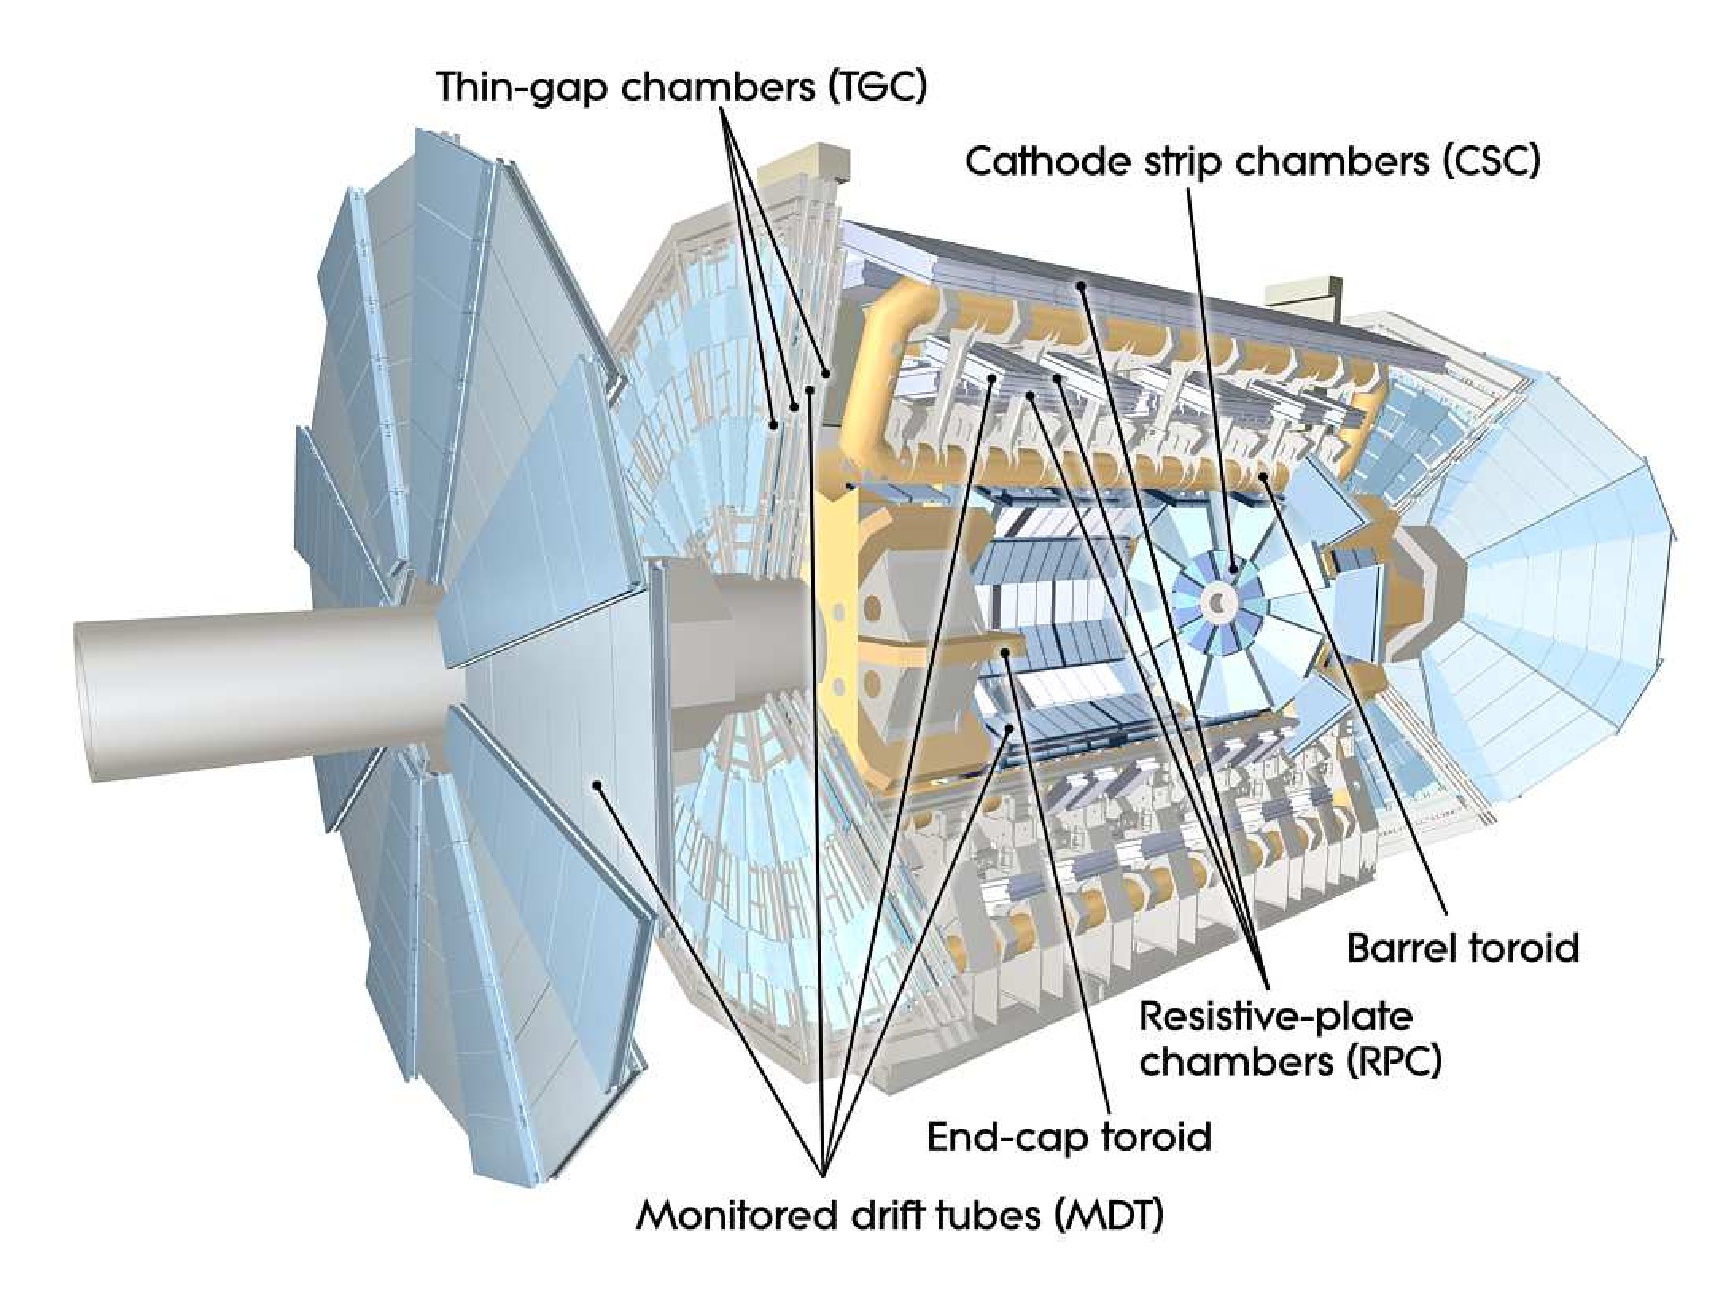
\includegraphics[width=0.7\textwidth]{figure/muonSpec.png}

    \end{center}
    \caption{Cut-away view of the ATLAS muon spectrometer system~\cite{ATLASDetector}.}



   \label{fig:atlasMu}
\end{figure}
The muon spectrometer is instrumented with separate high-precision tracking and muon trigger chambers. The measurement of the 
muon momenta is performed by reconstructing the  curvature of the muon trajectory in an intense toroidal magnetic field 
of 0.3-1.2\,T, which is  produced by the large superconducting air-core toroid magnets.
The layout of the muon spectrometer is shown in Figure~\ref{fig:atlasMu}.

Precision measurement of the track coordinates in the principal bending direction of the 
magnetic field is provided by three layers of Monitored Drift Tube chambers (MDT), covering the pseudorapidity range
 $|\eta| < 2.7\,.$ Given the high background rate at large pseudorapidities, 
$2 < |\eta| < 2.7$, the innermost MDT layer is replaced by the Cathode Strip Chambers (CSC). These are multi wire
proportional chambers with cathodes segmented into strips. 
The spectrometer allows for a precise muon momentum measurement for momenta up to 1~TeV.
The best momentum resolution of 3-4\% is achieved for muons with transverse momenta of about $100$~GeV, while resolution of 
about $10\%$ can be reached for muon momenta of 1~TeV. 

The trigger system covers the pseudorapidity range $|\eta| < 2.4\,.$ Resistive Plate Chambers
(RPC)  used in the barrel and Thin Gap Chambers (TGC) in the end-cap region
provide a relatively course but fast reconstruction of muon tracks needed  for the first-level muon trigger.


\subsection{The Trigger System}
For a detector like ATLAS, given the nominal LHC  bunch crossing rate of 40~MHz, it is technically impossible to record and store 
data for each bunch crossing. A  trigger system is therefore designed to reduce the initial rate to about 300~Hz, 
selecting only the interesting events. The triggering is performed in three stages with increasing selection power, the
so called  level~1 (L1), level~2 (L2), and the event filter (EF). Each trigger level
refines the decisions made at the previous level and, where necessary, applies additional selection
criteria.

The L1 trigger is hardware based and is designed to reach a decision within a latency of less than 2.5 $\mu$s, reducing the initial
rate to about 75~KHz. It  relies on coarse energy deposit in the calorimeter and muon trajectory in RPC and TGC chambers. It 
allows for the selection of high transverse-momentum muons, electrons, photons, jets, $\tau$ 
leptons decaying into hadrons, as well as large missing and total transverse energy.
The L1 trigger defines in each triggered event one or more regions of interest (RoI), i.e. the $\eta$ and $\phi$ coordinates
of detector regions in which a potential final state collision product is observed. %% BLEHA!!!

The L2 trigger  selection is seeded by the RoI information provided by the L1 trigger. Unlike the L1 trigger,
the L2 uses the full detector granularity in the given RoIs allowing for a more precise reconstruction of particle properties.
The L2 triggers are designed to reduce the trigger rate to approximately $3.5\,\text{kHz}$.

The final stage of the event selection is carried out by the event filter, which reduces
the event rate to roughly 300 Hz. Its selections are implemented 
applying reconstruction algorithms equivalent to the ones available offline. The offline reconstruction of 
physics object is described in Chapter~\ref{chap:obj}$\,$.


\subsection{Luminosity Measurement}
A precise measurement of the recordered instantaneous and integrated luminosity is a crucial ingredient of
all  physics studies at ATLAS.
Several luminosity measurement techniques are therefore employed as described in ~\cite{luminosity}.
The most relevant detectors for the luminosity monitoring are the inner detector,
the BMC~\cite{luminosity} and the LUCID~\cite{lucid} detectors. 
The inner detector provides the luminosity measurement from  the average number of reconstructed proton-proton interactions per bunch crossing.
The LUCID detector surrounds the beam pipe on both sides of the interaction point at a distance of 17 m. It consist of
Cherenkov detectors which  measure  the particle flux from the interaction point in a very forward region. The BCM detector 
consists of four small diamond sensors on each side of the interaction point arranged around the beam pipe in a cross pattern.
It is a fast device primarily designed to monitor the beam condition and can also provide an independent luminosity estimate.
The total uncertainty on the luminosity measurement obtained with these methods is about 3\%.










